\section{Auswertung}

Mit dem Ringmodulator wird die Amplitude eines Signals moduliert. Das Eingans- und Ausgangssignal sind in \autoref{a} zu sehen.

\begin{figure}
	\centering
	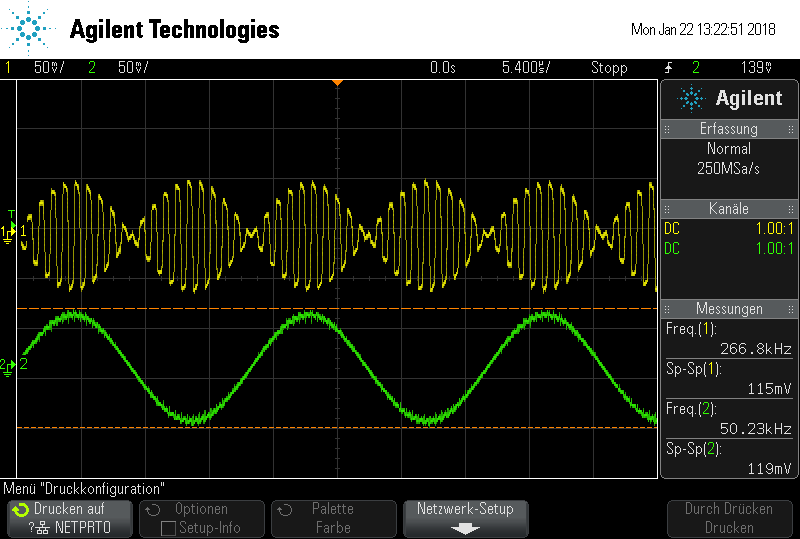
\includegraphics[width=\textwidth]{img/a_scope_230.png}
	\caption{Amplitudenmodulation - grün das Eingangssignal, gelb das amplitudenmodulierte Signal}
	\label{a}
\end{figure}

\begin{figure}
	\centering
	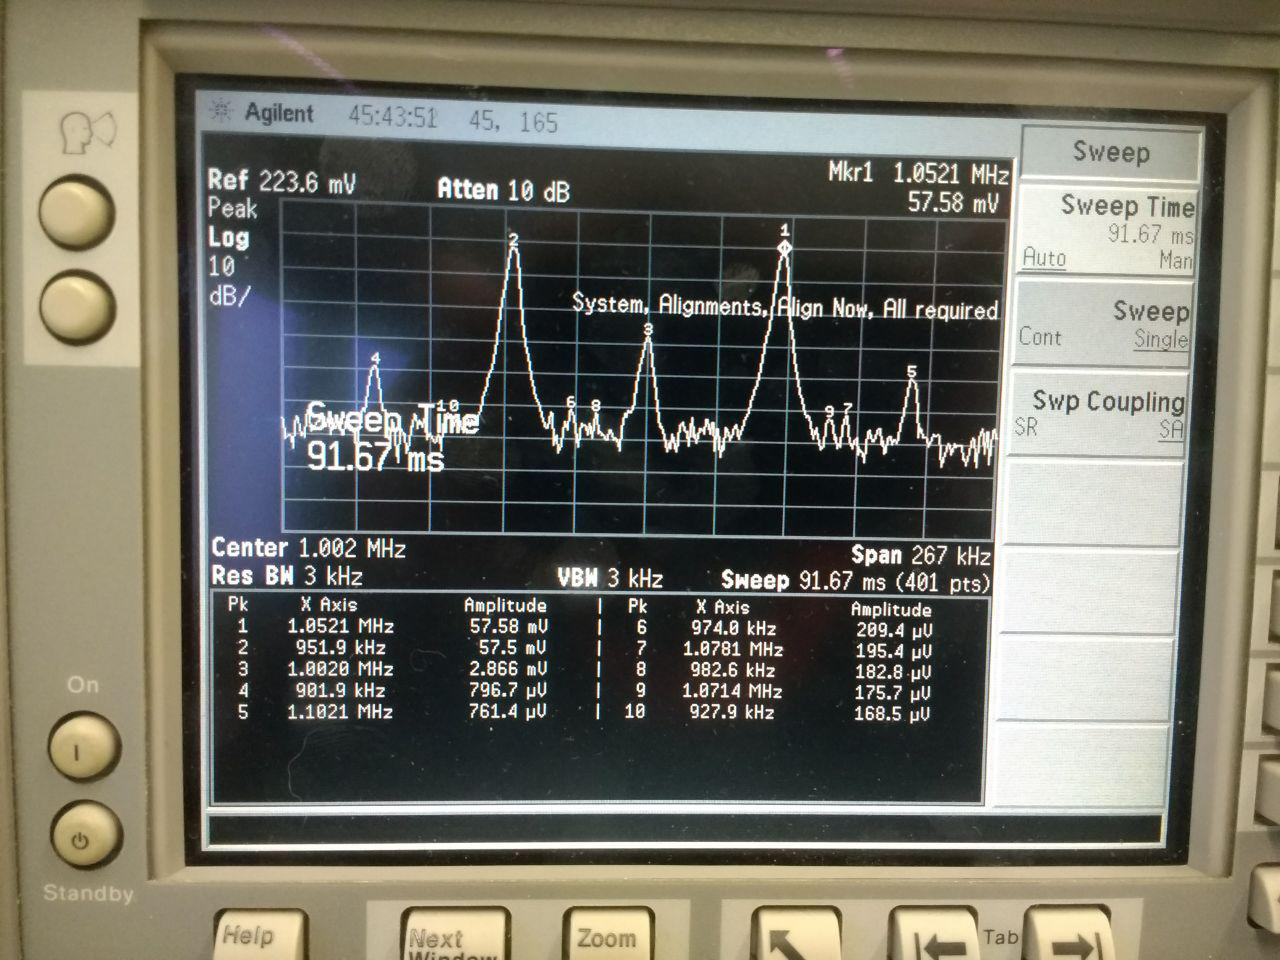
\includegraphics[width=\textwidth]{img/Aufgabenteil_b.jpg}
	\caption{Amplitudenmodulation - Peak 3 mit der Trägerfrequenz, Peak 1 und 2 die Seitenbänder}
\end{figure}

\begin{figure}[t!]
	\centering
	\begin{subfigure}[t]{0.5\textwidth}
		\centering
		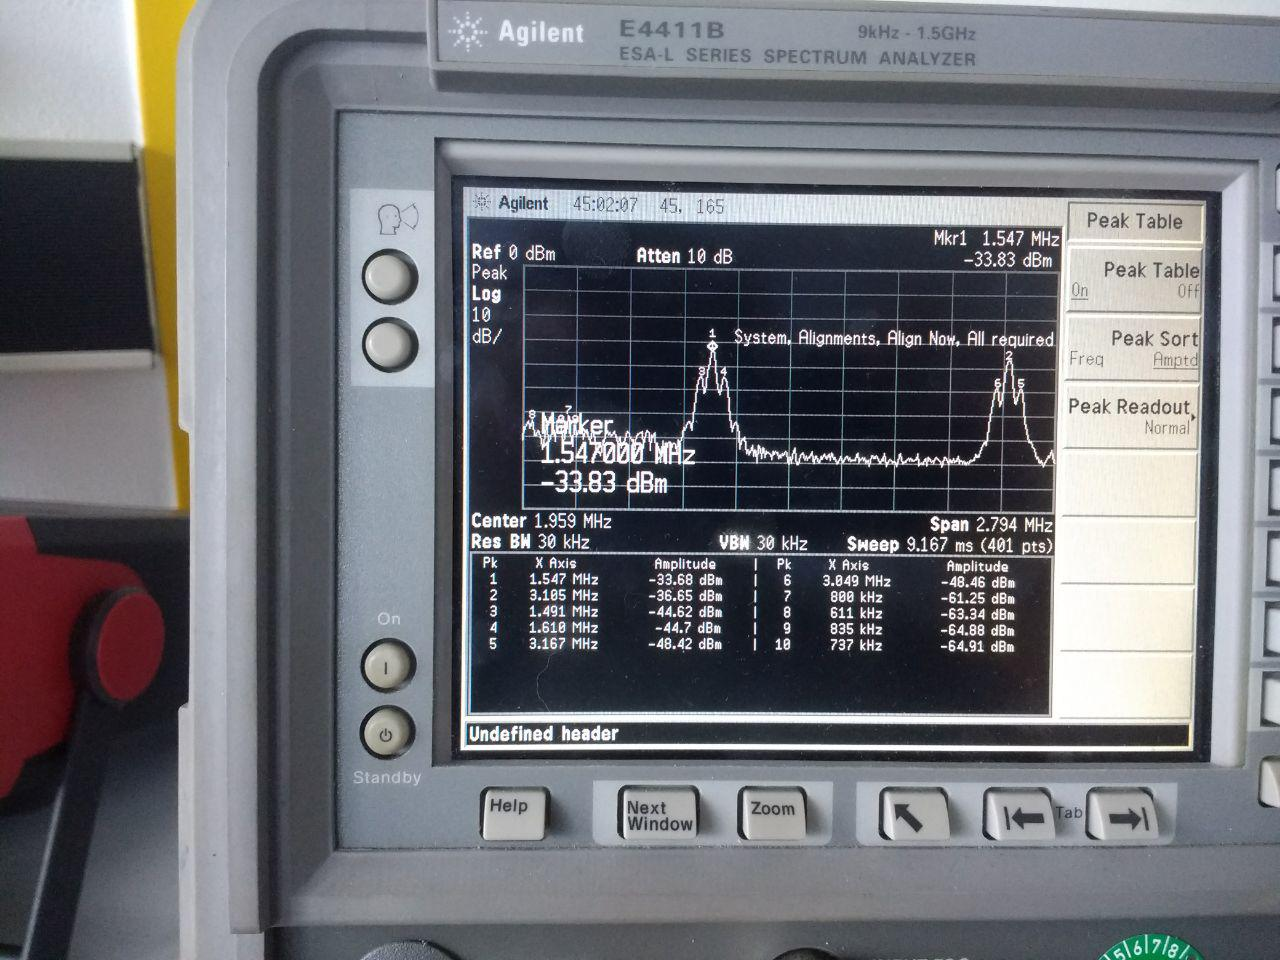
\includegraphics[width=\textwidth]{img/Aufgabenteil_c1.jpg}
		\caption{Amplitudenmodulation - mit Oberwellen}
	\end{subfigure}%
	~
	\begin{subfigure}[t]{0.5\textwidth}
		\centering
		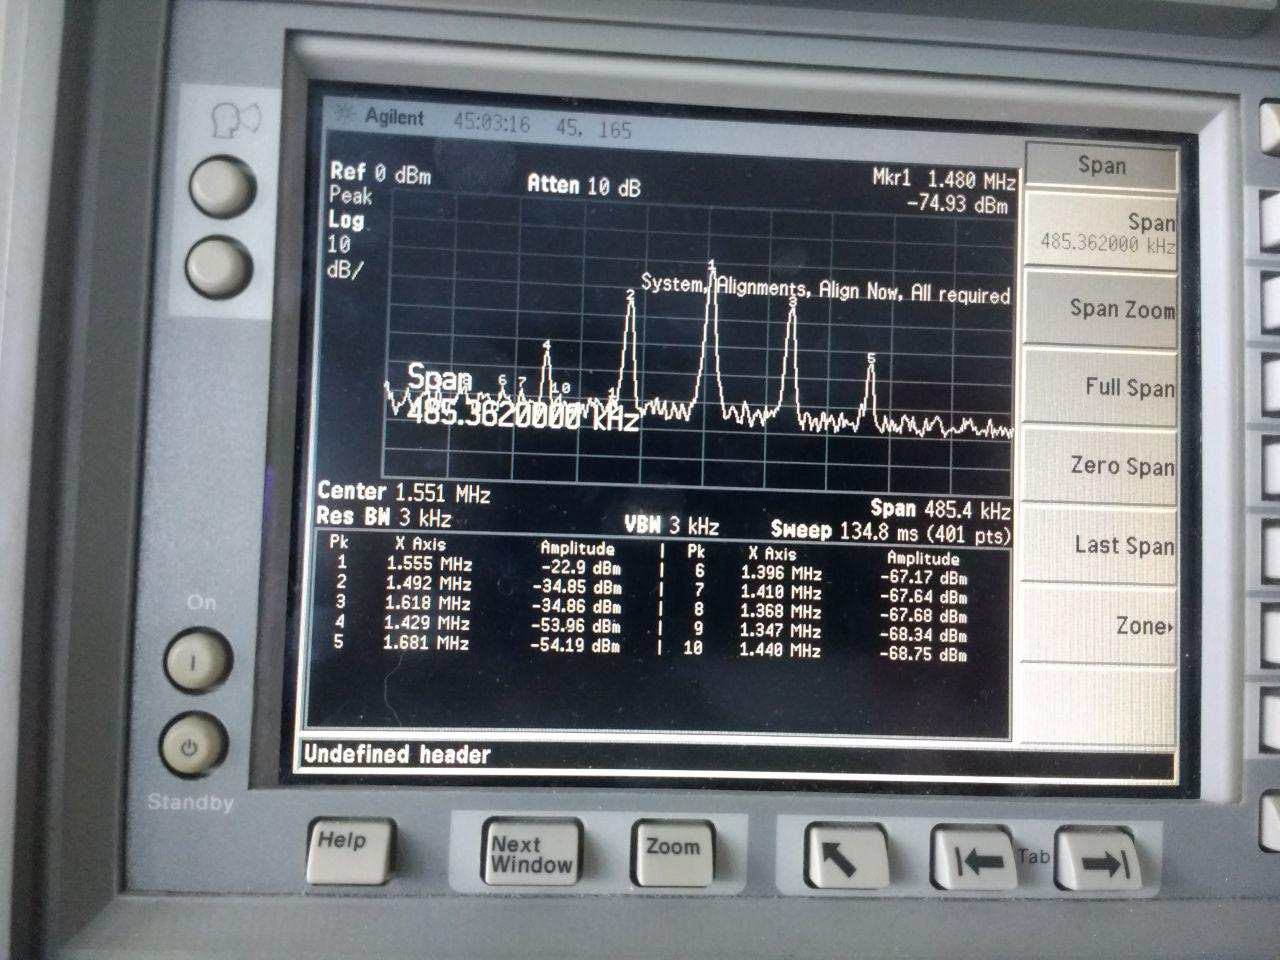
\includegraphics[width=\textwidth]{img/Aufgabenteil_c2.jpg}
		\caption{Amplitudenmodulation - Detailansicht}
	\end{subfigure}
\end{figure}

\begin{figure}
	\centering
	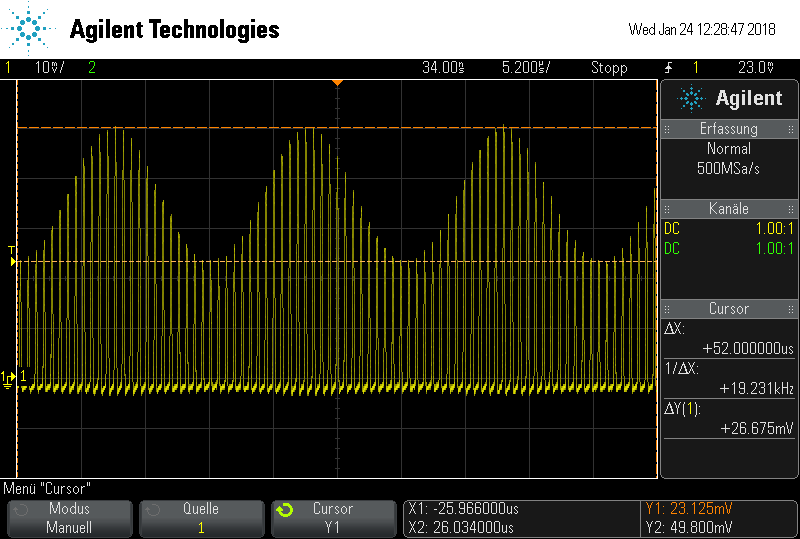
\includegraphics[width=\textwidth]{img/c_scope_247.png}
	\caption{Amplitudenmodulation - Bestimmung des Modulationsgrades}
\end{figure}

\begin{figure}[t!]
	\centering
	\begin{subfigure}[t]{0.5\textwidth}
		\centering
		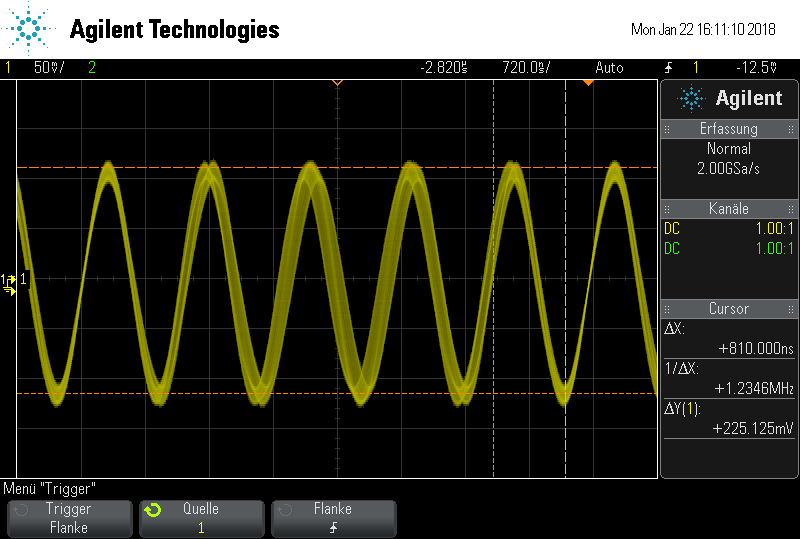
\includegraphics[width=\textwidth]{img/d_scope_233.png}
		\caption{Frequenzmodulation}
	\end{subfigure}%
	~
	\begin{subfigure}[t]{0.5\textwidth}
		\centering
		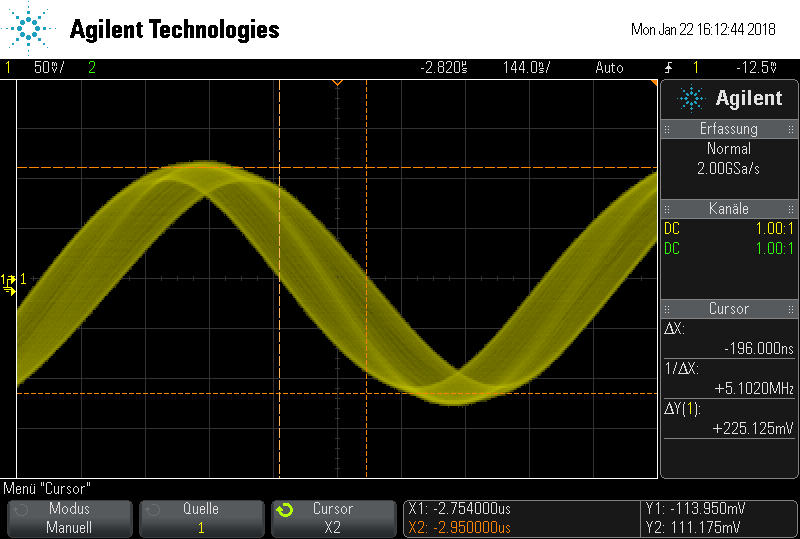
\includegraphics[width=\textwidth]{img/d_scope_234.png}
		\caption{Frequenzmodulation - Detailansicht}
	\end{subfigure}
\end{figure}

\begin{figure}
	\centering
	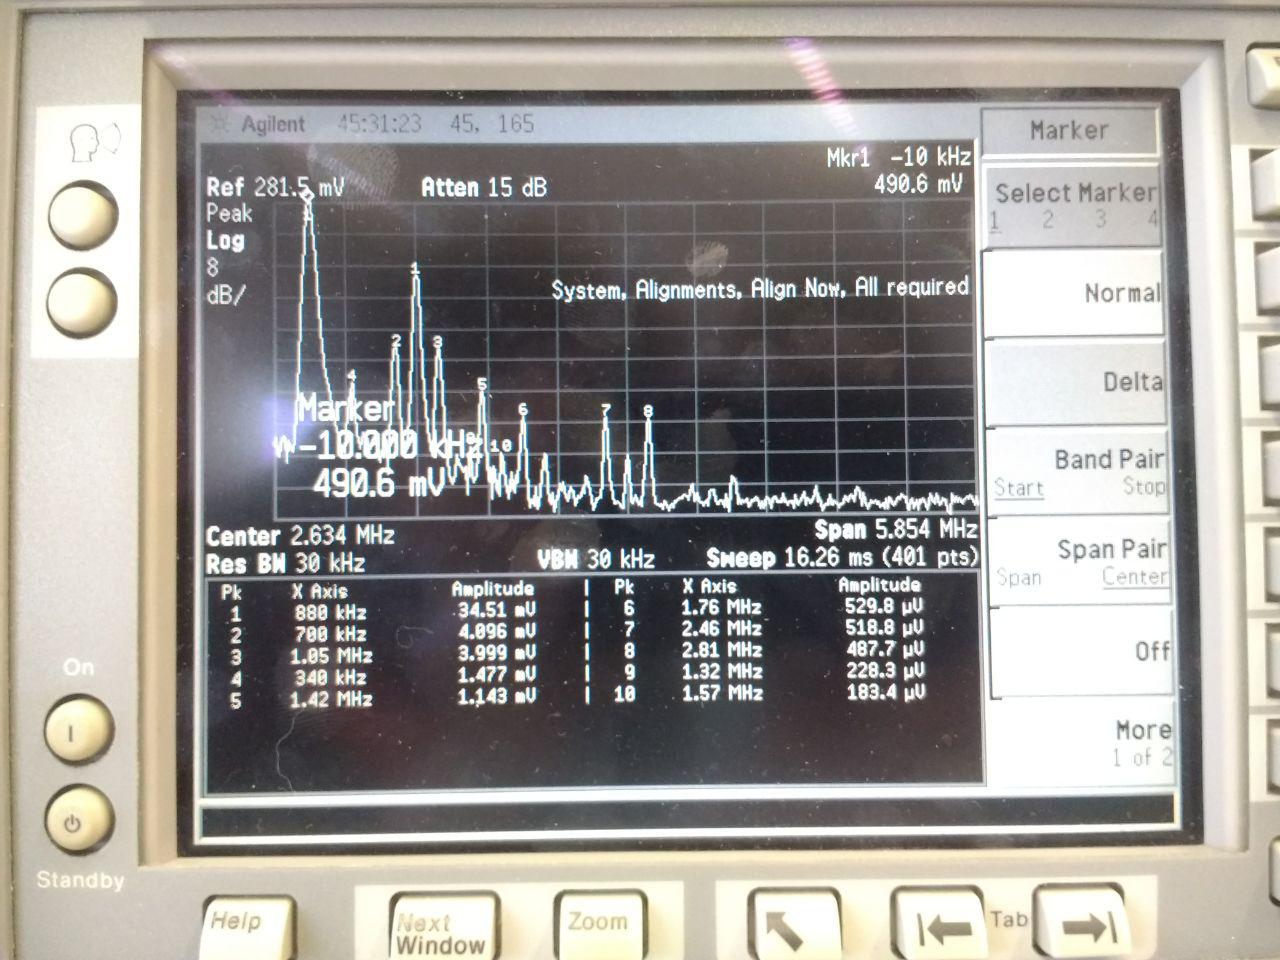
\includegraphics[width=\textwidth]{img/Aufgabenteil_d.jpg}
	\caption{Frequenzmodulation - Frequenzspektrum}
\end{figure}

\begin{figure}
	\centering
	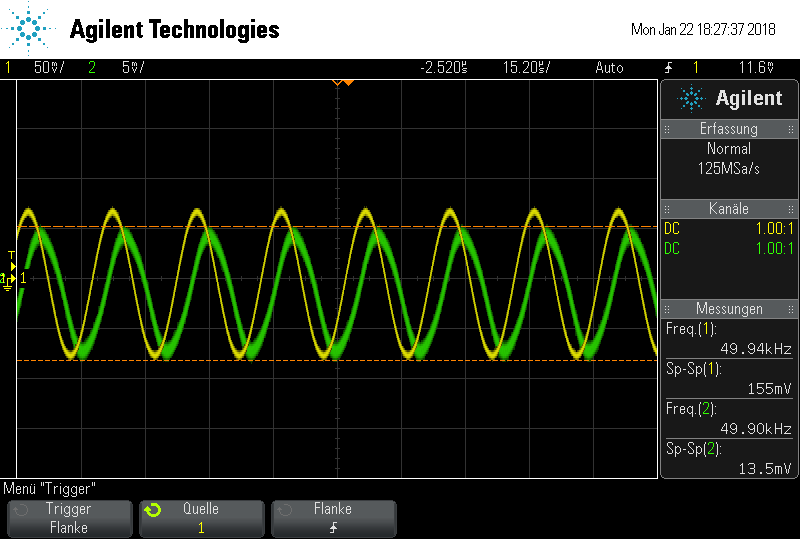
\includegraphics[width=\textwidth]{img/f_scope_235.png}
	\caption{Amplitudenmodulation - gelb das Eingangssignal, grün das amplitudenmodulierte und daraufhin demodulierte Signal}
\end{figure}

\begin{figure}[t!]
	\centering
	\begin{subfigure}[t]{0.5\textwidth}
		\centering
		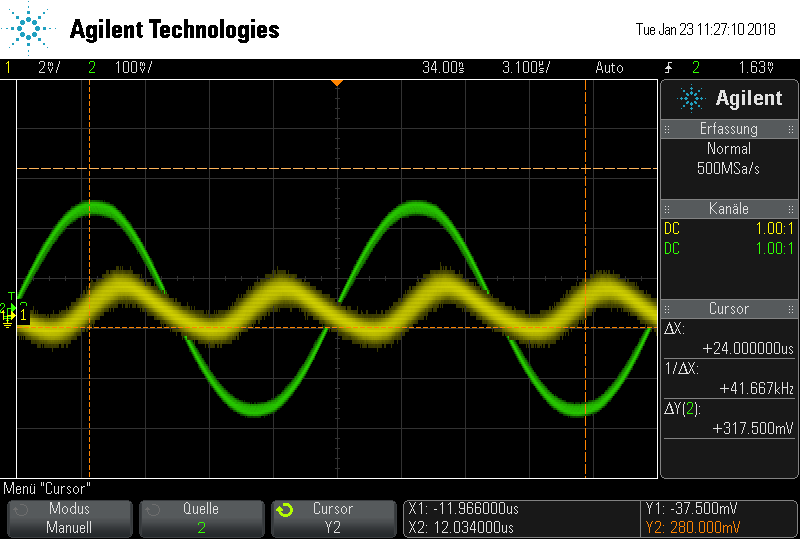
\includegraphics[width=\textwidth]{img/g_scope_242.png}
		\caption{Frequenzmodulation}
	\end{subfigure}%
	~
	\begin{subfigure}[t]{0.5\textwidth}
		\centering
		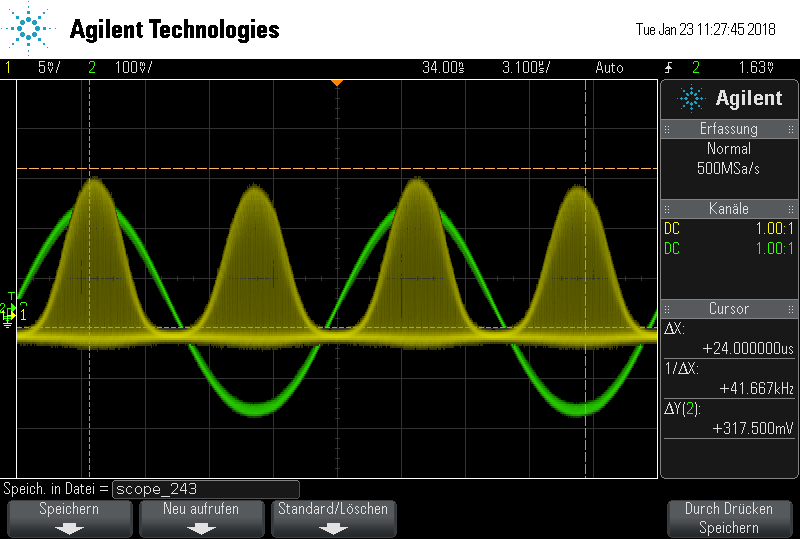
\includegraphics[width=\textwidth]{img/g_scope_243.png}
		\caption{Frequenzmodulation - Detailansicht}
	\end{subfigure}
\end{figure}

\begin{figure}[t!]
	\centering
	\begin{subfigure}[t]{0.5\textwidth}
		\centering
		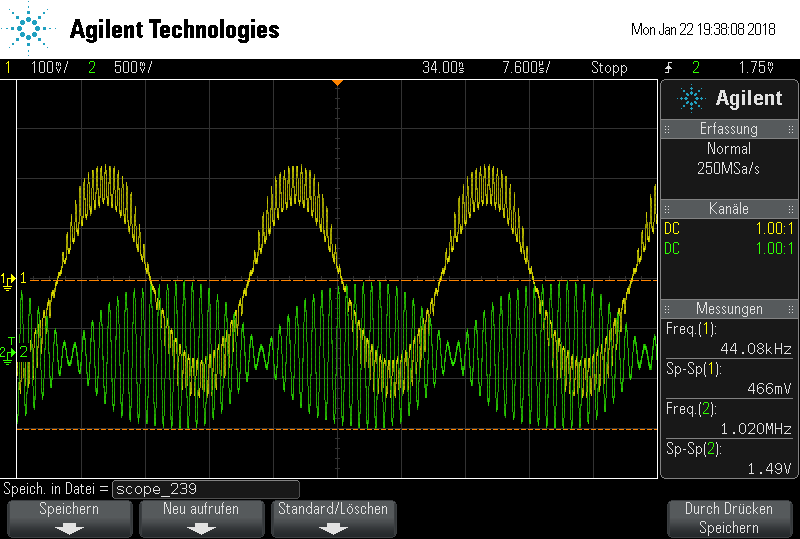
\includegraphics[width=\textwidth]{img/h_scope_239.png}
		\caption{Amplitudenmodulation - Amplitudenmodulation - moduliertes  Signal in grün, Eingangssignal in gelb}
	\end{subfigure}%
	~
	\begin{subfigure}[t]{0.5\textwidth}
		\centering
		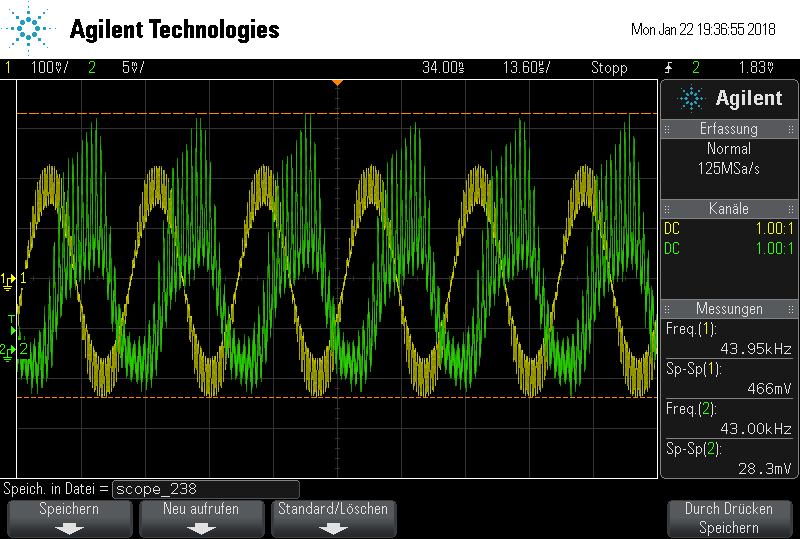
\includegraphics[width=\textwidth]{img/h_scope_238.png}
		\caption{Amplitudenmodulation - moduliertes und dann demoduliertes Signal in grün, Eingangssignal in gelb}
	\end{subfigure}
	\\
	\begin{subfigure}[t]{0.5\textwidth}
		\centering
		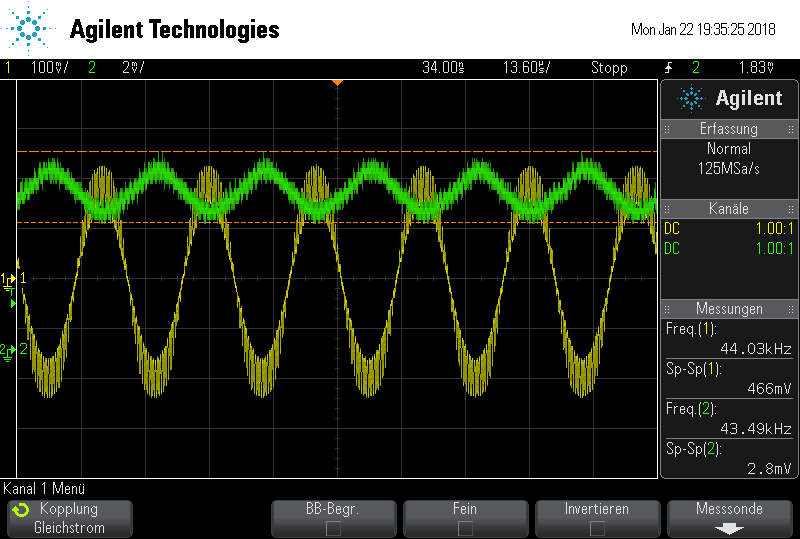
\includegraphics[width=\textwidth]{img/h_scope_237.png}
		\caption{Amplitudenmodulation - moduliertes und dann demoduliertes Signal nach Hochpass in grün, Eingangssignal in gelb}
	\end{subfigure}
\end{figure}

\FloatBarrier
